\clearpage
\section{典型例题与频谱分析}
\label{sec:ch2-worked-examples}

\noindent 以下例题沿用本章的傅里叶变换约定：
\[
    X(f)=\int_{-\infty}^{+\infty}x(t)e^{-\iu 2\pi ft}\diff t,
    \qquad \Omega=2\pi f\ \text{（谱角频率）},
    \qquad \Sa z=\frac{\sin z}{z},\quad \Sa 0=1.
\]
符号函数和阶跃函数需要用\textbf{广义傅里叶变换}处理；
普通傅里叶变换则根据全时间轴上的信号定义，选用积分法或性质法。

\subsection{例题1：正弦信号的绝对均值与方均根值}
\keypoint{复习重点：周期平均、绝对均值、均方值与方均根值的区别。}

\qs{正弦信号的时域特征参数}{
    求正弦信号 $x(t)=x_0\sin\omega t$ 的绝对均值和方均根值。
    设 $\omega>0$，周期为 $T_0=2\pi/\omega$。
}

\sol
\textbf{先写定义，再做一个周期的积分。}
绝对均值是信号绝对值在一个周期内的平均值，
方均根值是均方值的平方根。分别定义为
\[
    \mu_{|x|}=\frac{1}{T_0}\int_0^{T_0}|x(t)|\diff t,
    \qquad
    x_{\mathrm{rms}}=
    \sqrt{\frac{1}{T_0}\int_0^{T_0}x^2(t)\diff t}.
\]
令 $\theta=\omega t$，由 $\diff t=\diff\theta/\omega$ 得
\begin{align*}
    \mu_{|x|}
    &=\frac{|x_0|}{2\pi}
      \int_0^{2\pi}|\sin\theta|\diff\theta \\
    &=\frac{|x_0|}{2\pi}
      \left(\int_0^\pi\sin\theta\diff\theta
      -\int_\pi^{2\pi}\sin\theta\diff\theta\right)
      =\boxed{\frac{2|x_0|}{\pi}}.
\end{align*}
用 $\sin^2\theta=(1-\cos2\theta)/2$ 求均方值：
\begin{align*}
    \overline{x^2}
    &=\frac{x_0^2}{2\pi}\int_0^{2\pi}\sin^2\theta\diff\theta
      =\frac{x_0^2}{2}, \\
    x_{\mathrm{rms}}
    &=\sqrt{\overline{x^2}}
      =\boxed{\frac{|x_0|}{\sqrt{2}}}.
\end{align*}
若 $x_0>0$ 表示峰值，可直接写成
$\mu_{|x|}=2x_0/\pi$、$x_{\mathrm{rms}}=x_0/\sqrt{2}$。

\nt{
    \textbf{易错：绝对值放在积分内，不能放在积分外。}
    该正弦信号的普通均值为
    $\mu_x=T_0^{-1}\int_0^{T_0}x(t)\diff t=0$，
    因此 $|\mu_x|=0$，而 $\mu_{|x|}=2|x_0|/\pi$。
    因此，绝对均值 $\mu_{|x|}$ 与均值的绝对值 $|\mu_x|$ 是不同的量。
}

\ex{用特征参数检查答案}{
    对幅值不为零的正弦信号，峰值因数与波形因数分别为
    \[
        \frac{x_{\mathrm{peak}}}{x_{\mathrm{rms}}}=\sqrt{2},
        \qquad
        \frac{x_{\mathrm{rms}}}{\mu_{|x|}}
        =\frac{\pi}{2\sqrt{2}}\approx1.111.
    \]
    结果不随 $\omega$ 改变：频率决定每秒振荡次数，
    不改变完整周期内的幅值分布。
}

\subsection{例题2：单边指数衰减信号的频谱}
\keypoint{复习重点：由傅里叶变换定义求谱，并从复数形式提取幅值和相位。}

\qs{指数函数的幅频图与相频图}{
    设 $a>0$、$A\neq0$，单边指数衰减信号为
    $x(t)=Ae^{-at}u(t)$。
    求其频谱，并绘制幅频图与相频图。
}

\sol
当 $a>0$ 时，信号绝对可积，积分可直接计算：
\begin{align*}
    X(f)
    &=A\int_0^{+\infty}e^{-at}e^{-\iu2\pi ft}\diff t \\
    &=A\left[
        -\frac{e^{-(a+\iu2\pi f)t}}{a+\iu2\pi f}
      \right]_0^{+\infty}
      =\boxed{\frac{A}{a+\iu2\pi f}}.
\end{align*}
分母的实部恒为正，因此可不经过象限修正直接求分母相角。
令 $\alpha=\arg A$，选定一个相角值，则幅值和连续相位支为
\[
    \boxed{|X(f)|=\frac{|A|}{\sqrt{a^2+(2\pi f)^2}}},
    \qquad
    \boxed{\phi(f)=\alpha-\arctan\frac{2\pi f}{a}}.
\]
图中按这一连续相位支绘制；若需主值相位，可按 $2\pi$ 周期折回。
绘图时抓住三个位置即可：
\begin{itemize}
    \item $f=0$：$X(0)=A/a$，幅值最大，为 $|A|/a$；相位为 $\alpha$。
    \item $f=\pm a/(2\pi)$：幅值为 $|A|/(\sqrt{2}a)$；
          相位分别为 $\alpha\mp\pi/4$。
    \item $f\to\pm\infty$：幅值趋于 $0$；
          相位分别趋于 $\alpha\mp\pi/2$。
\end{itemize}

\begin{center}
    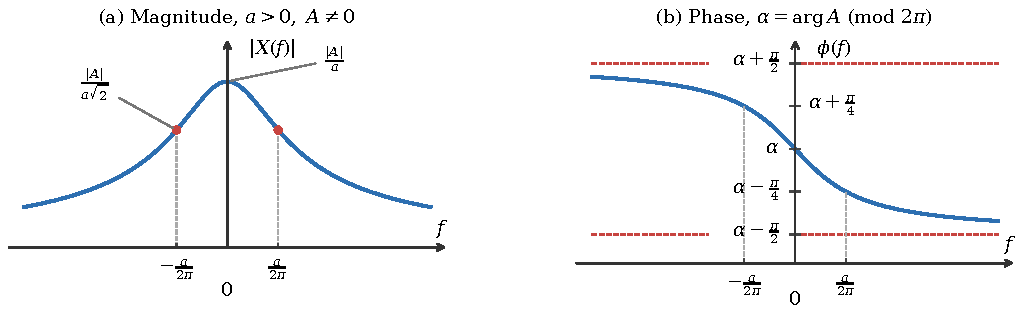
\includegraphics[width=.98\linewidth]{hw02-exponential.pdf}
\end{center}

幅频图始终关于纵轴对称，连续相位支满足
$\phi(-f)=2\alpha-\phi(f)$。
当 $A$ 为实数时，信号才为实信号，满足 $X(-f)=X^*(f)$。
其中 $A>0$ 对应 $\alpha=0$，相位为
$\phi(f)=-\arctan(2\pi f/a)$，是关于原点对称的特例。
将零频幅值归一化后，谱宽由 $a$ 决定：
$a$ 越大，时域衰减越快，归一化幅频图越宽。

\nt{
    \textbf{易错：单边指数信号的负时间区间为零；横轴单位必须统一。}
    若去掉 $u(t)$，把 $Ae^{-at}$ 定义在全时间轴上，
    它在 $t\to-\infty$ 时发散，
    上述普通傅里叶积分不成立。
    用谱角频率写时为 $A/(a+\iu\Omega)$，
    改用 $f$ 后必须代入 $\Omega=2\pi f$。
    当 $A$ 为负实数时，可取 $\alpha=\pi$，再按所需主值区间折回相位；
    $A=0$ 时相位没有定义。
}

\Needspace{5cm}
\subsection{例题3：符号函数与单位阶跃函数的广义频谱}
\keypoint{复习重点：微分性质、冲激项、主值分布及其谱图表示。}

\qs{符号函数与阶跃函数}{
    求 $\sgn(t)$ 与 $u(t)$ 的频谱，
    使用频率 $f$ 为横坐标绘制幅频图与相频图。
    采用 $\sgn(0)=0$、$u(0)=1/2$ 的对称约定。
}

\sol
这两个信号不绝对可积，不能把普通积分当作收敛积分计算。
引入主值符号 $\PV$，用对称方式处理 $f=0$ 附近的奇性。
\textbf{以下变换等式在广义函数意义下成立。}

\subsubsection{符号函数：用微分性质确定连续部分}
\[
    \sgn(t)=
    \begin{cases}
        -1,&t<0,\\
        1,&t>0,
    \end{cases}
    \qquad
    \frac{\diff}{\diff t}\sgn(t)=2\delta(t).
\]
设 $S(f)=\mathcal F\{\sgn(t)\}$。由
$\mathcal F\{x'(t)\}=\iu2\pi fX(f)$、
$\mathcal F\{\delta(t)\}=1$ 得
\[
    \iu2\pi fS(f)=2.
\]
在 $f\neq0$ 时，$S(f)=1/(\iu\pi f)$。
微分式本身不能排除 $C\delta(f)$，因为 $f\delta(f)=0$；
但 $\sgn(t)$ 是实奇函数，其频谱必须为纯虚奇分布，
不能含偶的 $\delta(f)$ 项。因此
\[
    \boxed{\mathcal F\{\sgn(t)\}
    =\PV\!\left(\frac{1}{\iu\pi f}\right)}.
\]
也可用收敛信号验证这个结果。令
$s_\varepsilon(t)=\sgn(t)e^{-\varepsilon|t|}$，$\varepsilon>0$，则
\begin{align*}
    \mathcal F\{s_\varepsilon(t)\}
    &=\frac{1}{\varepsilon+\iu2\pi f}
      -\frac{1}{\varepsilon-\iu2\pi f} \\
    &=\frac{-\iu4\pi f}{\varepsilon^2+(2\pi f)^2}
      \xrightarrow[\varepsilon\downarrow0]{\text{广义极限}}
      \PV\!\left(\frac{1}{\iu\pi f}\right).
\end{align*}

\subsubsection{单位阶跃：由符号函数补齐零频冲激}
利用 $u(t)=[1+\sgn(t)]/2$ 与 $\mathcal F\{1\}=\delta(f)$，可得
\[
    \boxed{U(f)=\mathcal F\{u(t)\}
    =\frac12\delta(f)
      +\PV\!\left(\frac{1}{\iu2\pi f}\right)}.
\]
这里 $\delta(f)/2$ 来自阶跃的常值分量。
若只对 $u'(t)=\delta(t)$ 做变换，
得到 $\iu2\pi fU(f)=1$，会漏掉微分消去的零频项；
所以必须另外确定冲激的系数。

\subsubsection{如何画幅频与相频示意图}
对 $f\neq0$，频谱是通常的复数函数，因而可以写
\[
    |S(f)|=\frac{1}{\pi|f|},
    \qquad
    |U_{\mathrm c}(f)|=\frac{1}{2\pi|f|},
\]
其中 $U_{\mathrm c}$ 表示阶跃谱的连续部分。两者相位相同：
\[
    \phi(f)=
    \begin{cases}
        +\pi/2,&f<0,\\
        -\pi/2,&f>0.
    \end{cases}
\]

\begin{center}
    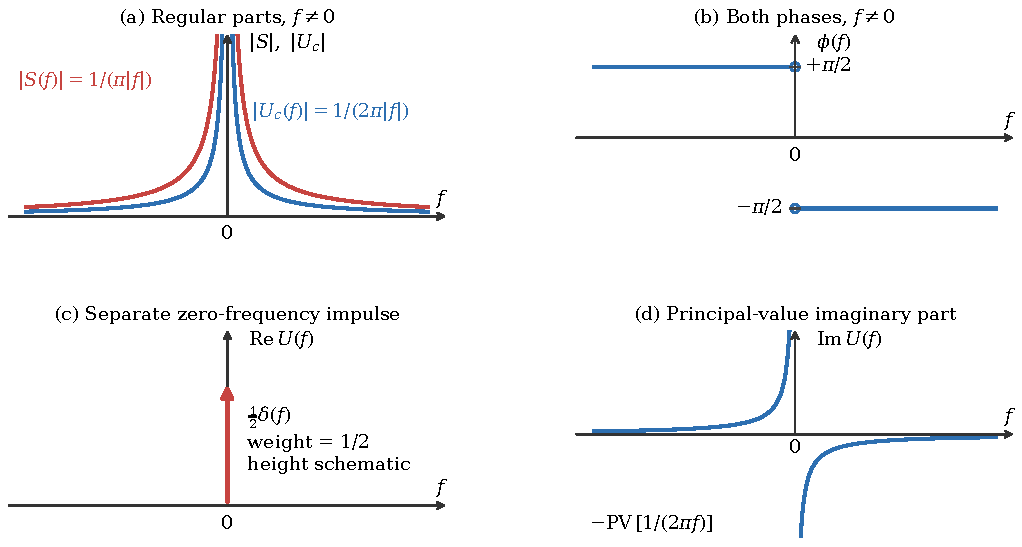
\includegraphics[width=.98\linewidth]{hw03-generalized.pdf}
\end{center}

\nt{
    \textbf{易错：广义频谱不能在 $f=0$ 处直接取模。}
    图中的曲线仅表示 $f\neq0$ 的连续部分；
    阶跃谱在 $f=0$ 处还须单独画一个冲激箭头，标注\textbf{权重 $1/2$}。
    箭头长度不是有限的冲激高度，也不能把
    $|\delta(f)/2+1/(\iu2\pi f)|$ 当作普通函数计算。
    $f=0$ 的整个广义频谱不具有普通“幅值、相位”数值。
    符号函数的奇性是主值项，不能误画成额外的零频冲激。
}

\subsection{例题4：截断余弦与两个平移的矩形窗频谱}
\keypoint{复习重点：矩形窗变换、调制性质、幅频与有符号频谱的区别。}

\qs{被截断余弦的傅里叶变换}{
    求
    \[
        y(t)=
        \begin{cases}
            \cos2\pi f_0t,&|t|\leq T,\\
            0,&|t|>T
        \end{cases}
    \]
    的傅里叶变换，并以 $f$ 为横坐标绘制频谱。
    其中 $T>0$，截断窗口总宽度为 $2T$。
}

\sol
\textbf{先求窗谱，再搬移到 $\pm f_0$。}
令 $w(t)=1$（$|t|\leq T$），其余处为 $0$，则
$y(t)=w(t)\cos2\pi f_0t$。
\begin{align*}
    W(f)
    &=\int_{-T}^{T}e^{-\iu2\pi ft}\diff t \\
    &=\frac{e^{\iu2\pi fT}-e^{-\iu2\pi fT}}{\iu2\pi f}
      =\frac{\sin2\pi fT}{\pi f}
      =2T\Sa(2\pi fT).
\end{align*}
$f=0$ 处由极限补上 $W(0)=2T$。利用欧拉公式与频移性质：
\begin{align*}
    y(t)
    &=\frac12w(t)e^{\iu2\pi f_0t}
      +\frac12w(t)e^{-\iu2\pi f_0t},\\
    Y(f)
    &=\frac12W(f-f_0)+\frac12W(f+f_0).
\end{align*}
\[
    \boxed{Y(f)=T\Sa\bigl(2\pi T(f-f_0)\bigr)
       +T\Sa\bigl(2\pi T(f+f_0)\bigr)}.
\]
这也等价于把两条理想余弦谱线
$[\delta(f-f_0)+\delta(f+f_0)]/2$
分别与 $W(f)$ 卷积。

为绘制两个平移分量，记
\[
    Y_+(f)=T\Sa\bigl(2\pi T(f-f_0)\bigr),
    \qquad
    Y_-(f)=T\Sa\bigl(2\pi T(f+f_0)\bigr).
\]
下图分别画出 $Y_+(f)$ 和 $Y_-(f)$，竖线用于定位各自的中心频率。
$Y_+$ 在 $f=f_0$ 处峰高为 $T$，首零点为 $f_0\pm1/(2T)$；
$Y_-$ 在 $f=-f_0$ 处峰高为 $T$，首零点为 $-f_0\pm1/(2T)$。
这些峰和零点均属于\textbf{单个分量}；真正的总谱必须逐点代数相加：
$Y(f)=Y_+(f)+Y_-(f)$。

\begin{center}
    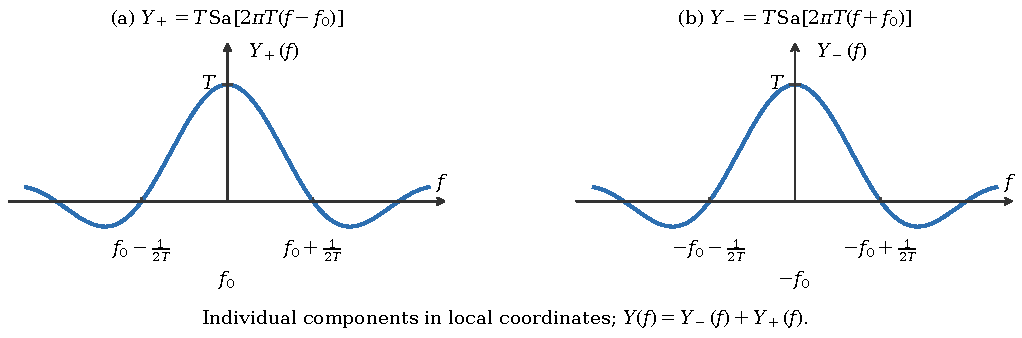
\includegraphics[width=.98\linewidth]{hw04-windowed.pdf}
\end{center}

\textbf{总频谱的幅值与相位。}
因为 $y(t)$ 为实偶函数，$Y(f)$ 也是实偶函数，
但其旁瓣可取负值。
幅频图应画 $|Y(f)|$；有符号的频谱图则保留负旁瓣。相位为
\[
    \phi(f)=
    \begin{cases}
        0,&Y(f)>0,\\
        \pi\quad(\mathrm{mod}\ 2\pi),&Y(f)<0,
    \end{cases}
\]
$Y(f)=0$ 处相位无定义。

每个平移的窗谱以 $\pm f_0$ 为中心，
自身的第一对零点距中心为 $1/(2T)$，
所以每个主瓣的零点间宽度为 $1/T$。
这是\textbf{各个分量}的零点和宽度，
叠加后总频谱的零点、峰值位置还受到另一分量的影响。
例如
\[
    Y(0)=2T\Sa(2\pi f_0T),
    \qquad
    Y(f_0)=T\bigl[1+\Sa(4\pi f_0T)\bigr].
\]
仅在另一个窗谱的贡献较小时，才可近似把载频处的峰高视为 $T$。

\nt{
    \textbf{易错：截断并未保留两条理想谱线。}
    时域相乘对应频域卷积，有限窗口把谱线展宽为带旁瓣的连续谱。
    $T$ 是半窗宽，窗口频谱为 $2T\Sa(2\pi fT)$，
    不能误写成 $T\Sa(\pi fT)$。
    窗越长，主瓣越窄；两个平移的窗谱需要先做\textbf{代数相加}，
    再取绝对值，不能把两个窗谱的模直接相加。
    两端点取不取等号不影响傅里叶积分。
}

\Needspace{8cm}
\subsection{例题5：指数衰减振荡的频谱与实际峰位}
\keypoint{复习重点：指数谱频移、复数合并与幅频峰的位置。}

\qs{指数衰减振荡信号}{
    设 $a>0$、$\omega>0$，指数衰减振荡信号为
    $x(t)=e^{-at}\sin\omega t\,u(t)$。
    利用单边指数信号的频谱及傅里叶变换性质，求其频谱，
    并以 $f$ 为横坐标绘制幅频图。
}

\sol
令 $g(t)=e^{-at}u(t)$，单边指数信号的变换为
$G(f)=1/(a+\iu2\pi f)$。
设振荡频率 $f_{\mathrm s}=\omega/(2\pi)$，由
$\sin\omega t=(e^{\iu\omega t}-e^{-\iu\omega t})/(2\iu)$ 得
\begin{align*}
    X(f)
    &=\frac{1}{2\iu}\bigl[G(f-f_{\mathrm s})-G(f+f_{\mathrm s})\bigr]\\
    &=\frac{1}{2\iu}
      \left[
        \frac{1}{a+\iu(2\pi f-\omega)}
        -\frac{1}{a+\iu(2\pi f+\omega)}
      \right]\\
    &=\boxed{\frac{\omega}{(a+\iu2\pi f)^2+\omega^2}}.
\end{align*}
把分母分成实部和虚部，得到幅频表达式
\[
    \boxed{
    |X(f)|=
    \frac{\omega}
    {\sqrt{\bigl[a^2+\omega^2-(2\pi f)^2\bigr]^2
    +4a^2(2\pi f)^2}}
    }.
\]
该幅值是偶函数，零频处为
$|X(0)|=\omega/(a^2+\omega^2)$。

\subsubsection{峰值并不总在 $\pm\omega/(2\pi)$}
令 $q=(2\pi f)^2\geq0$。幅值最大等价于其分母平方最小：
\begin{align*}
    D(q)
    &=(a^2+\omega^2-q)^2+4a^2q\\
    &=q^2+2(a^2-\omega^2)q+(a^2+\omega^2)^2,\\
    D'(q)&=2(q+a^2-\omega^2).
\end{align*}
因此，
\[
    \boxed{
    f_{\mathrm{peak}}=
    \begin{cases}
        \displaystyle\pm\frac{\sqrt{\omega^2-a^2}}{2\pi},
            &\omega>a,\\[2mm]
        0,&0<\omega\leq a.
    \end{cases}}
\]
当 $\omega>a$ 时，存在两个对称峰，峰高为 $1/(2a)$；
当 $\omega\leq a$ 时，最大值在中心，峰高为
$\omega/(a^2+\omega^2)$。
弱衰减 $a\ll\omega$ 时，双峰才接近 $\pm\omega/(2\pi)$。

绘制幅谱时，先标出中心值 $\omega/(a^2+\omega^2)$、上述峰位和峰高，
再利用关于纵轴的对称性补齐曲线。
下图分别示意 $\omega>a$ 的双峰与 $0<\omega\leq a$ 的中心单峰。

\begin{center}
    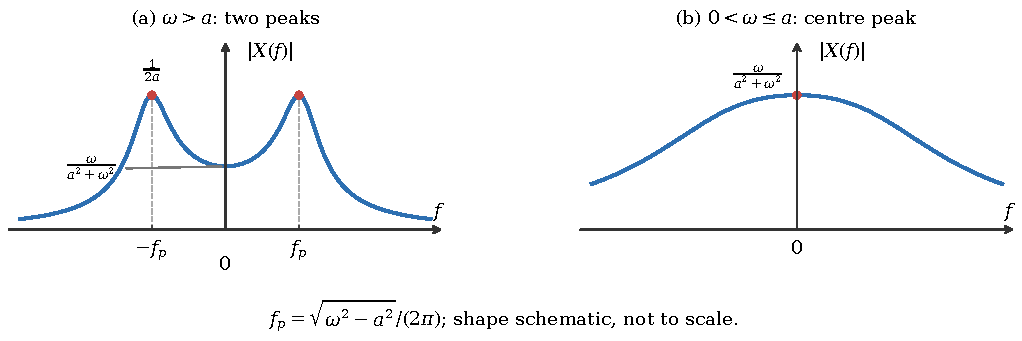
\includegraphics[width=.98\linewidth]{hw05-damped.pdf}
\end{center}

\nt{
    \textbf{易错：两次频移后的复数谱要先相减，再取模。}
    不能把 $|X(f)|$ 画成两个指数幅频图的简单叠加，
    也不能因正弦的名义频率是 $\omega$ 就把最大值固定在 $\pm\omega$。
    这里横轴为 $f$，频率位置均须除以 $2\pi$。
    若省略 $u(t)$ 而把原式定义在整条实轴上，
    负时间方向会指数增长，普通傅里叶积分不收敛。
}

\subsection{例题6：余弦调制与频谱搬移、重叠}
\keypoint{复习重点：欧拉展开的 $1/2$ 系数、两个搬移副本及频带重叠条件。}

\qs{调幅信号与载波频率的关系}{
    设 $m(t)$ 为实值调制信号，其频谱为 $M(f)$，满足带限模型
    \[
        M(f)=0\quad(|f|>f_m),
        \qquad f_m=\frac{\omega_m}{2\pi}>0.
    \]
    采用角频率为 $\omega_0>0$ 的余弦载波，记
    \[
        f_{\mathrm c}=\frac{\omega_0}{2\pi},
        \qquad s(t)=m(t)\cos\omega_0t.
    \]
    求调幅信号 $s(t)$ 的傅里叶变换，示意画出时域和频域信号，
    并讨论 $\omega_0>\omega_m$、$\omega_0=\omega_m$
    与 $\omega_0<\omega_m$ 时的频带关系。
}

\sol
利用欧拉公式展开载波，再应用频移性质：
\begin{align*}
    s(t)
    &=\frac12m(t)e^{\iu2\pi f_{\mathrm c}t}
      +\frac12m(t)e^{-\iu2\pi f_{\mathrm c}t}.
\end{align*}
\[
    \boxed{S(f)=\frac12M(f-f_{\mathrm c})
        +\frac12M(f+f_{\mathrm c})}.
\]
两项分别把原谱搬到正、负载频处，
每个副本都乘 $1/2$，谱形保持不变。
若改用谱角频率 $\Omega$ 为横轴，定义
$\mathcal M(\Omega)=M(\Omega/2\pi)$、
$\mathcal S(\Omega)=S(\Omega/2\pi)$，则同一结论写作
\[
    \boxed{\mathcal S(\Omega)
      =\frac12\mathcal M(\Omega-\omega_0)
       +\frac12\mathcal M(\Omega+\omega_0)}.
\]

\subsubsection{时域图：快速振荡受调制信号控制}
对于实信号，$|s(t)|\leq|m(t)|$。
可先画 $m(t)$ 的形状，再在其内部画载波振荡；
若 $m(t)\geq0$，上下包络为 $\pm m(t)$。
一般情况下，幅值包络为 $|m(t)|$，
$m(t)$ 改变正负号时还会使载波翻转 $\pi$ 相位。
该调制信号没有额外的常值载波项，
是双边带抑制载波调制的基本形式。

下图根据给定的 $m(t)$ 轮廓，在包络内画出载波振荡，
并将一般的 $M(f)$ 轮廓左右平移以构造调制频谱。
时域包络与频谱轮廓为形状示意；
频带端点和每个副本的 $1/2$ 系数由变换公式决定。

\begin{center}
    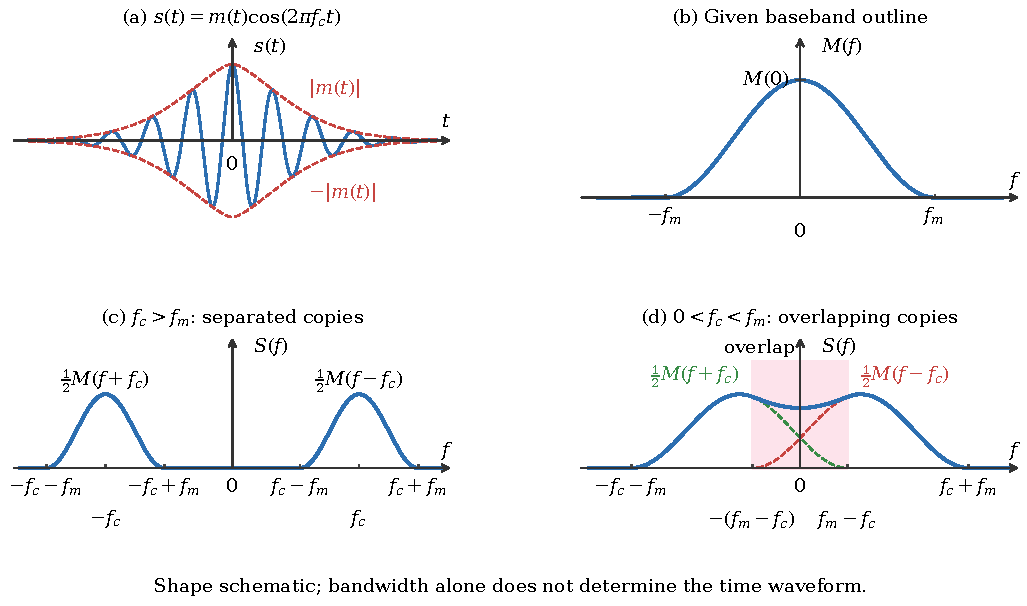
\includegraphics[width=.98\linewidth]{hw06-modulation.pdf}
\end{center}

\subsubsection{频域图：按频带端点判断是否重叠}
在 $M(f)=0$（$|f|>f_m$）的带限模型下，
两个频谱副本分别位于以下频带范围内：
\[
    I_+=[f_{\mathrm c}-f_m,\ f_{\mathrm c}+f_m],
    \qquad
    I_-=[-f_{\mathrm c}-f_m,\ -f_{\mathrm c}+f_m].
\]
\begin{itemize}
    \item $f_{\mathrm c}>f_m$：两副本分离，
          中间间隔宽度为 $2(f_{\mathrm c}-f_m)$，
          等价于 $\omega_0>\omega_m$。
    \item $f_{\mathrm c}=f_m$：两频带在 $f=0$ 处恰好相接；
          边界处是否有非零值，取决于原谱端点。
    \item $0<f_{\mathrm c}<f_m$：两频带范围重叠，交集为
          \[
              I_+\cap I_-
              =[-(f_m-f_{\mathrm c}),\ f_m-f_{\mathrm c}],
          \]
          重叠宽度为 $2(f_m-f_{\mathrm c})$。
          用角频率表示，区间为
          $[-(\omega_m-\omega_0),\ \omega_m-\omega_0]$。
\end{itemize}
重叠区内两个复数谱相加。
当两个副本在同一频率处均非零时，不能只靠带通滤波把它们单独分离。
对于非严格带限、但能量主要集中在 $|f|\leq f_m$ 内的实际信号，
$f_m$ 可作为有效带宽；此时上述条件描述的是\textbf{主要频带}是否重叠，
频带外的谱尾仍可能有贡献。

\nt{
    \textbf{易错：重叠区仍按同一变换公式计算，且系数始终为 $1/2$。}
    $\omega_0<\omega_m$ 不会使频移性质失效，
    只是两个副本在同一频率处发生叠加。
    “不能靠带通分离副本”也不等于“任何方法都无法恢复原信号”；
    恢复能力还取决于所用方法及信号的额外信息。
    时域相乘引起频域搬移，时域平移则引起相位因子，二者不可混用。
}
